\documentclass[twocolumn,prd,amsmath,amssymb,aps,superscriptaddress,nofootinbib]{revtex4-2}

\usepackage{graphicx}
\usepackage{dcolumn}
\usepackage{bm}
\usepackage{hyperref}
\usepackage{color}
\usepackage{mathtools}
\usepackage{booktabs}
\usepackage{amsfonts}
\usepackage{tikz} % For figures

\begin{document}

\title{Gravity Derived: Emergence from Information Constraints}

\author{Jonathan Washburn}
\affiliation{Independent Researcher, Austin, Texas}

\date{\today}

\begin{abstract}
\noindent
Gravity emerges from finite information–bandwidth constraints on the substrate that maintains gravitational fields. We derive a phenomenological weight law $w(r)=\lambda\,\xi\,n(r)\,(T_{\text{dyn}}/\tau_0)^\alpha\,\zeta(r)$ from an optimization principle under finite bandwidth. Coefficients are fixed once, globally (no per–galaxy tuning). We present the conceptual foundations, the mathematical derivation, and a summary of empirical validation on SPARC rotation curves; full statistics and figures appear in the companion paper \cite{Washburn2025a}.
\end{abstract}

\maketitle

\section{Introduction}

For over three centuries, gravity has stood as physics' most familiar yet mysterious force. Newton provided the mathematical description, Einstein revealed the geometric nature, but neither explained why mass warps spacetime or attracts other mass. The discovery of galactic rotation anomalies \cite{Rubin1970} and cosmic acceleration \cite{Riess1998} has only deepened the mystery, spawning exotic solutions like dark matter particles and dark energy fields that together comprise 95\% of the universe yet remain undetected.

The dark matter paradigm, despite decades of searches, has yielded no direct detection. Experiments spanning 90 orders of magnitude in mass---from ultralight axions to primordial black holes---have found nothing. The parameter space for WIMPs, once the leading candidate, shrinks with each null result from ever-more-sensitive detectors. Meanwhile, simulations predict far more satellite galaxies than observed (the missing satellites problem), cuspy dark matter profiles that observations reject (the core-cusp problem), and struggle to explain the observed diversity of rotation curves (the diversity problem).

Modified gravity theories like MOND \cite{Milgrom1983} fare better empirically, reproducing galactic dynamics with remarkable economy. Yet MOND itself poses deep puzzles. Why should nature care about a particular acceleration scale $a_0 \approx 10^{-10}$ m/s$^2$? How can a modification designed for galaxies also predict aspects of cosmology? Most troublingly, MOND's empirical success lacks a compelling theoretical foundation---it works too well to be wrong, yet no one knows why it works at all.

This work explores an alternative perspective inspired by information-theoretic approaches to physics \cite{Wheeler1990, Lloyd2002}. Building on ideas from holographic principles \cite{tHooft1993, Susskind1995} and entropic gravity \cite{Verlinde2011, Jacobson1995}, we propose that gravitational phenomena emerge from constraints on information processing in a fundamental substrate. Unlike Verlinde's entropic gravity, which derives forces from thermodynamic gradients on holographic screens, or Jacobson's thermodynamic derivation of the Einstein field equations, our framework focuses on dynamic bandwidth limitations in field updates, leading to a distinct, optimization-based derivation of the MOND acceleration scale and galactic dynamics without per–galaxy tuning. We refer to this non‑relativistic limit as Information‑Limited Gravity (ILG).

Consider the computational challenge gravity presents. With $\sim 10^{80}$ particles in the observable universe, maintaining gravitational interactions requires processing an astronomical amount of information. Every mass must know about every other mass, fields must update as objects move, and all this must happen consistently across scales from subatomic to cosmic. No finite system could manage this exactly.

In this paper, we derive gravity from first principles by recognizing that any system maintaining consistent gravitational interactions across cosmic scales faces severe information-theoretic constraints. Just as a computer operating system must allocate limited CPU cycles among competing processes, the substrate maintaining gravitational fields must manage finite bandwidth.

This bandwidth limitation, we argue, is not a mere analogy but the fundamental origin of gravitational phenomena. Systems requiring frequent updates (like solar systems with short orbital periods) consume more bandwidth and thus receive priority. Systems evolving slowly (like galaxies with $\sim$100-million-year rotation periods) can tolerate delayed updates. This "refresh lag" between field updates creates the phenomena we observe as dark matter and dark energy.

The paper now proceeds as follows: Section I revisits the informational foundations; Section II derives gravity from the bandwidth optimisation principle; Section III analyses the emergent acceleration scale and unification of dark matter/energy; Section IV explores quantum and cosmological connections; Section V outlines qualitative empirical support, referring readers to the companion observational paper; we conclude in Section VI.

\section{Foundational Premises}
\label{sec:foundations}

\subsection{Reality as Information Processing}

Following Wheeler's "it from bit" and recent developments in quantum information theory, we begin with the premise that reality fundamentally consists of information processing rather than material substance. This is not merely philosophical speculation---the holographic principle, black hole thermodynamics, and quantum error correction in AdS/CFT all point toward information as the fundamental currency of physics.

Key principle: Physical laws emerge from optimal information processing under constraints.

\subsection{The Substrate and Its Constraints}

Any system processing information faces three universal constraints that shape its behavior. First, finite bandwidth limits information transmission according to channel capacity, as formalized by the Shannon-Hartley theorem. Second, finite memory means that state storage requires physical resources, whether quantum states, classical bits, or more exotic representations. Third, optimization pressure ensures that limited resources must be allocated efficiently to maximize global utility.

We remain agnostic about the nature of this information-processing substrate, which may emerge from holographic degrees of freedom at spacetime boundaries \cite{Susskind1995} or quantum computational limits \cite{Lloyd2002}. The key insight is that regardless of its ultimate nature, any such substrate faces these constraints when maintaining gravitational fields across the universe.

The constraints become particularly severe when we consider the scale of the gravitational computation. With approximately $10^{80}$ particles in the observable universe, each potentially interacting with every other, the information processing requirements are staggering. Even restricting to gravitationally significant masses leaves an overwhelming computational burden that any finite system must manage through intelligent resource allocation.

\subsection{The Bandwidth Bottleneck}

Consider the computational demands of gravity. Every mass must interact with every other mass, leading to $N^2$ scaling in computational complexity. Fields must continuously update as objects move through space, maintaining consistency across all scales from subatomic to cosmic. Furthermore, information cannot propagate faster than light, imposing fundamental limits on update synchronization.

For a universe with $\sim 10^{80}$ particles, maintaining exact Newtonian gravity would require $\sim 10^{160}$ pairwise force calculations per update cycle. This is computationally prohibitive for any finite system.

\subsection{The Triage Solution}

Faced with overwhelming computational demands, any intelligent system would implement triage---prioritizing urgent updates while delaying less critical ones. We propose this is exactly what occurs in nature.

Solar systems receive the highest priority for updates due to their orbital periods ranging from days to years. The risk of collisions and complex N-body dynamics demand frequent attention. These systems update every fundamental update cycle, preserving Newtonian gravity to high precision.

Galaxy disks occupy a medium priority tier. With rotation periods around $10^8$ years and stable, quasi-circular orbits, they can tolerate less frequent updates. We propose they refresh approximately every 100 cycles, creating the apparent extra gravity we attribute to dark matter.

The cosmic web receives the lowest priority. Its expansion timescale of $\sim 10^{10}$ years and slow, predictable dynamics allow updates only every $\sim$1000 cycles. This sparse updating modifies the expansion dynamics, manifesting as what we call dark energy.

This triage naturally emerges from optimizing global utility under bandwidth constraints. The substrate allocates its limited resources where they matter most---preventing collisions, maintaining orbital stability, and ensuring large-scale coherence---while economizing where possible.

\section{Derivation of Gravitational Law}
\label{sec:derivation}

\subsection{Information Content of Gravitational Fields}

The gravitational field configuration for $N$ masses requires specifying complete information about the field at every point in space. This includes the field vector at each spatial location, comprising three directional components multiplied by the spatial resolution of our discretization. The field must be specified with sufficient precision to distinguish physically relevant differences in gravitational strength. Additionally, temporal consistency must be maintained across update cycles to ensure conservation laws remain satisfied.

The total information content of a gravitational field is bounded holographically \cite{Bekenstein1973, tHooft1993}, scaling with surface area rather than volume:
\begin{equation}
I_{\text{field}} \leq 3 \times \left(\frac{L^2}{\ell_{\text{min}}^2}\right) \times \log_2\left(\frac{g_{\text{max}}}{g_{\text{min}}}\right) \times N_{\text{interactions}}
\end{equation}

This formula captures several key aspects. The factor of 3 accounts for the three spatial components of the gravitational field vector. The term $(L/\ell_{\text{min}})^2$ reflects an area (holographic) bound on degrees of freedom at resolution $\ell_{\text{min}}$. The logarithmic term $\log_2(g_{\text{max}}/g_{\text{min}})$ quantifies the bits needed to represent the dynamic range of the field strength. Finally, $N_{\text{interactions}}$ accounts for the number of significant mass interactions contributing to the field. The resulting requirement is enormous, motivating optimization under finite bandwidth rather than exact refresh everywhere.

\subsection{Channel Capacity Constraints}

The total information flow for gravitational updates cannot exceed channel capacity:
\begin{equation}
\sum_{\text{systems}} \frac{I_{\text{system}}}{\Delta t_{\text{system}}} \leq B_{\text{total}}
\end{equation}
where $B_{\text{total}}$ is the total available bandwidth and $\Delta t_{\text{system}}$ is the refresh interval for each system.

\subsection{Optimization Problem}

The substrate must solve:
\begin{align}
\text{maximize: } & \sum_i U_i(\Delta t_i) \quad \text{[total utility]} \
\text{subject to: }\\ & \sum_i \frac{I_i}{\Delta t_i} \leq B_{\text{total}} \quad \text{[bandwidth constraint]}
\end{align}
where $U_i$ represents the "utility" of updating system $i$ frequently.

Natural utility function: $U_i = -K_i \times \Delta t_i^\alpha$ where $K_i$ is the urgency factor (collision risk, dynamical complexity), $\alpha$ is the diminishing returns exponent, and the negative sign ensures longer delays reduce utility.

\subsection{Utility Function Selection}

What utility function should the substrate use? Consider physical requirements. Shorter delays are always preferred: $dU/d\Delta t < 0$. Diminishing returns apply: $d^2U/d\Delta t^2 < 0$. Scale invariance requires: $U(k\Delta t) = k^\alpha U(\Delta t)$.

These constraints suggest:
\begin{equation}
U_i(\Delta t_i) = -K_i \Delta t_i^\alpha
\end{equation}
where $K_i$ represents the "urgency" of system $i$.

To see why this form emerges naturally, consider the general scale-invariant utility satisfying our constraints. Any such function must satisfy the functional equation:
\begin{equation}
U(\lambda \Delta t) = f(\lambda) U(\Delta t)
\end{equation}
for some function $f$. Taking derivatives with respect to $\lambda$ and setting $\lambda = 1$ yields:
\begin{equation}
\Delta t U'(\Delta t) = f'(1) U(\Delta t)
\end{equation}
This differential equation has the general solution $U(\Delta t) = C \Delta t^{\alpha}$ where $\alpha = f'(1)$. The requirement that utility decreases with delay ($dU/d\Delta t < 0$) implies $\alpha > 0$ and $C < 0$, giving our form with $C = -K_i$.

The exponent $\alpha$ is fixed by the scale‑invariant utility together with the eight‑tick ledger symmetry, yielding
\[
  \alpha \,=\, \tfrac12\Bigl(1 - \tfrac{1}{\varphi}\Bigr)\;\approx\;0.191\;,
\]
with convexity requiring $\alpha<2$. No empirical calibration enters this value.

For a constructive proof sketch and formal context, see the Recognition Science framework (self‑similarity and golden‑ratio section) where the eight‑tick ledger symmetry forces the continued‑fraction recursion converging to $\varphi$.

Physical factors affecting urgency include collision risk for systems with crossing orbits, dynamical complexity from N-body chaos and resonances, observable importance for systems hosting observers, and energy density where high-energy regions need accuracy.

\subsection{Lagrangian Solution}

Using Lagrange multipliers:
\begin{equation}
\mathcal{L} = \sum_i (-K_i \Delta t_i^\alpha) - \mu\left(\sum_i \frac{I_i}{\Delta t_i} - B_{\text{total}}\right)
\end{equation}

Taking derivatives:
\begin{equation}
\frac{\partial \mathcal{L}}{\partial \Delta t_i} = -\alpha K_i \Delta t_i^{\alpha-1} + \mu \frac{I_i}{\Delta t_i^2} = 0
\end{equation}

Solving for optimal refresh interval:
\begin{equation}
\Delta t_i^* = \left(\frac{\mu I_i}{\alpha K_i}\right)^{1/(2-\alpha)}
\end{equation}

This reveals the key scaling: systems with larger information content $I_i$ receive longer refresh intervals, while urgent systems (high $K_i$) receive shorter intervals.

\subsection{Recognition Weight Function}

The refresh lag creates a mismatch between the actual field and ideal Newtonian field. We define the information weight as:
\begin{equation}
w = \frac{\text{effective gravity}}{\text{Newtonian gravity}}
\end{equation}

During the interval $\Delta t$ between updates, objects continue moving while fields remain static. For circular orbits, this creates an effective boost:
\begin{equation}
w \approx 1 + \frac{v \Delta t}{r} \approx 1 + \frac{\Delta t}{T_{\text{dyn}}}
\end{equation}
where $T_{\text{dyn}} = 2\pi r/v$ is the dynamical time.

To understand this physically, consider a star orbiting in a galaxy. At time $t_0$, the gravitational field is updated based on the mass distribution. The star experiences the correct force and begins its orbital motion. However, the field remains frozen until the next update at $t_0 + \Delta t$. During this interval, the star has moved to a new position, but continues experiencing the force from its original location. This mismatch between where the star is and where the field "thinks" it is creates an apparent extra force.

For slow-moving systems where $\Delta t \ll T_{\text{dyn}}$, this effect is negligible---the star barely moves between updates. But in galaxies where $\Delta t \sim T_{\text{dyn}}$, the star completes a significant fraction of its orbit between updates. The accumulated error manifests as additional centripetal acceleration, exactly mimicking the effect of extra unseen mass. This is why dark matter appears to trace visible matter so perfectly---it's not a coincidence but a direct consequence of refresh lag scaling with the visible mass distribution.

\subsection{Emergent Acceleration Scale}

The transition between Newtonian and modified regimes occurs when refresh lag becomes significant:
\begin{equation}
\Delta t \sim T_{\text{dyn}}
\end{equation}

For galaxies with $\Delta t \sim 10^8$ years:
\begin{equation}
T_{\text{dyn}} \sim 10^8 \text{ years} \rightarrow \frac{v^2}{r} \sim 10^{-10} \text{ m/s}^2
\end{equation}

This naturally produces the MOND acceleration scale $a_0 \simeq 1.2\times10^{-10}\,\mathrm{m\,s^{-2}}$ without fine‑tuning.

\subsection{Physical Interpretation of the Emergent Scale}

The emergence of a characteristic acceleration scale $a_0 \sim 10^{-10}$ m/s$^2$ from our bandwidth framework deserves deeper examination. This scale has puzzled physicists since Milgrom first identified it empirically in 1983. Why should gravity "know" about this particular acceleration?

In our framework, $a_0$ represents the acceleration at which refresh lag effects become comparable to the dynamical time. Below this acceleration, systems evolve so slowly that even infrequent updates suffice to maintain approximate Newtonian behavior. Above this acceleration, rapid dynamics demand frequent updates that the bandwidth-limited substrate can provide.

The numerical value of $a_0$ emerges from the intersection of several cosmic timescales. The age of the universe sets the overall temporal context. The fundamental update cycle time, derived from the Recognition framework's eight‑tick cycle, determines the fundamental update frequency. The typical refresh interval for galactic systems, emerging from optimization under bandwidth constraints, provides the final ingredient. When these timescales combine, they naturally produce an acceleration scale matching observations.

This explains why $a_0$ appears universal despite arising from a complex optimization process. The bandwidth constraints and utility functions are themselves universal, leading to consistent resource allocation patterns across different systems. Just as the speed of light emerges as a universal limit from special relativity, $a_0$ emerges as a universal scale from bandwidth-limited gravity.

Furthermore, this interpretation makes testable predictions. Systems with unusual complexity or dynamics should show deviations from the standard $a_0$ value. Young galaxies at high redshift, with different evolutionary histories, might exhibit slightly different transition scales. These predictions distinguish our framework from MOND, where $a_0$ is simply postulated as fundamental.

\section{Complete Mathematical Formalism}
\label{sec:formalism}

\subsection{Information Weight Definition}

Combining all factors, the information weight becomes:
\begin{equation}
w(r) = \lambda \times \xi \times n(r) \times \left(\frac{T_{\text{dyn}}}{\tau_0}\right)^\alpha \times \zeta(r)
\end{equation}

Each component serves a distinct physical purpose. The global normalization $\lambda$ enforces bandwidth conservation across the universe, ensuring that the total computational resources allocated to gravitational updates remain finite; we take $\lambda = 1/(2\,\varphi^3) \approx 0.118$ with $\varphi = (1+\sqrt5)/2$. The complexity factor $\xi$ captures how system dynamics affect update priority, with more complex systems earning more frequent refreshes. The spatial refresh profile $n(r)$ describes how update frequency varies within a single galaxy, allowing the model to capture radial variations in refresh lag. The dynamical time scaling $(T_{\text{dyn}}/\tau_0)^\alpha$ emerges directly from the Lagrangian optimization, encoding how slowly evolving systems tolerate longer refresh intervals; we use the fundamental tick $\tau_0 = 7.33\times10^{-15}\,\mathrm{s}$. Finally, the geometric correction $\zeta(r)$ accounts for deviations from idealized thin‑disk assumptions.

\subsection{Complexity Factor}

Systems with complex dynamics require more frequent updates, formalized through:
\begin{equation}
\xi = 1 + C_0 f_{\text{gas}}^\gamma \left(\frac{\Sigma_0}{\Sigma_*}\right)^\delta
\end{equation}

This expression captures multiple aspects of galactic complexity. The gas fraction $f_{\text{gas}}$ serves as a proxy for turbulent, star-forming activity that demands computational attention. Gas-rich systems host active star formation, turbulent flows, and rapid dynamical evolution---all requiring frequent field updates. The central surface brightness $\Sigma_0$ indicates the overall activity level, with brighter centers typically hosting more vigorous dynamics. The reference scale $\Sigma_* = 10^8 M_\odot$/kpc$^2$ provides dimensional consistency.

Our optimization yields specific values for these parameters: $C_0 = 5.064$ controls the overall strength of complexity boosting, $\gamma = 2.953$ determines how strongly gas content affects priority, and $\delta = 0.216$ governs the surface brightness dependence. The near-cubic scaling with gas fraction ($\gamma \approx 3$) suggests that complexity scales with the volume of turbulent gas, consistent with three-dimensional turbulent cascade theories.

\noindent\textit{Inputs and provenance.} We take $f_{\rm gas}$ from SPARC mass models (gas to total baryonic mass fraction within the optical radius) and $\Sigma_0$ as the central surface brightness from the same catalogs; $\Sigma_*$ is a fixed reference $10^8\,M_\odot/\mathrm{kpc}^2$. All inputs are computed once per galaxy and held fixed across model comparisons to ensure like-for-like evaluation.

\noindent\textit{Sensitivity.} Varying $(C_0,\gamma,\delta)$ by $\pm10\%$ changes median $\chi^2/N$ at the few-percent level, with the strongest response to $\gamma$; see robustness discussion in Sec.~\ref{sec:qualitative}. A full sweep appears in the companion paper.

\noindent\textit{Explicit definitions.} We use
\begin{align}
  f_{\rm gas} &= \frac{M_{\rm gas}^{\rm (HI+H_2)}}{M_{\rm gas}^{\rm (HI+H_2)} + M_\star}\;,\\
  \Sigma_0 &= \frac{M_\star}{2\pi R_d^2}\;,
\end{align}
with $R_d$ estimated from the radius at which the disk contribution peaks (\,$\simeq\,2.2 R_d$\,). These quantities are derived once per galaxy by the SPARC master-table build (Sec.~\ref{sec:code}) and reused identically across ILG, MOND, and NFW evaluations.

\subsection{Spatial Profile}

The function $n(r)$ captures how refresh priority varies within a galaxy. For transparency and reproducibility we use a closed‑form, monotonic profile
\begin{equation}
  n_{\mathrm{analytic}}(r)\;=\;1 + A\Bigl[1 - \exp\!\bigl(-(r/r_0)^p\bigr)\Bigr],
  \label{eq:n-analytic}
\end{equation}
with $(A, r_0, p) = (7,\,8\,\mathrm{kpc},\,1.6)$ fixed once, globally (no per–galaxy tuning). This captures the observed transition from inner to outer regions while avoiding spline control‑point choices.
Operationally, $n(r)$ models the radial refresh‑lag envelope that arises from longer orbital times and disk geometry, and is not a mass model or fit per galaxy.

\subsection{Geometric correction}
\label{sec:zeta}

The factor $\zeta(r)$ captures geometric deviations from thin, axisymmetric disks (e.g., flaring, warp, thickness). We bound it as $\zeta\in[0.9,1.1]$ for typical late-type disks and take $\zeta(r)=1$ unless independently indicated by geometry (warp) flags in the catalog. Sensitivity to $\zeta$ within this band is subdominant compared to $n(r)$ changes and is included in the robustness sweep.

\subsection{Dynamical Time Factor}

The dynamical time dependence emerges from the Lagrangian optimization:
\begin{equation}
\left(\frac{T_{\text{dyn}}}{\tau_0}\right)^\alpha \quad \text{with} \quad T_{\text{dyn}} = \frac{2\pi r}{v_{\text{obs}}}
\end{equation}

Fixed value: $\alpha = 0.191$ (derived from $\varphi$; see Sec.~\ref{sec:derivation})

The modest exponent indicates robust bandwidth allocation---not extreme triage but consistent prioritization.

\subsection{Modified Rotation Curve}

The observed rotation velocity becomes:
\begin{equation}
v_{\text{model}}^2(r) = w(r) \times v_{\text{baryon}}^2(r)
\end{equation}
where $v_{\text{baryon}}^2 = v_{\text{gas}}^2 + v_{\text{disk}}^2 + v_{\text{bulge}}^2$ is the Newtonian prediction.

This simple multiplication by $w(r)$ transforms failing Newtonian predictions into accurate fits.

\section{Constants and Notation}
\label{sec:notation}

For convenience we list fixed constants and recurring symbols:
\begin{center}
\begin{tabular}{ll}
\toprule
Symbol & Meaning \\
\midrule
$\alpha$ & Exponent in $U(\Delta t)=-K\,\Delta t^{\alpha}$; $\alpha=\tfrac12(1-1/\varphi)\approx0.191$ \\
$\lambda$ & Global normalization; $\lambda=1/(2\,\varphi^3)\approx0.118$ \\
$\tau_0$ & Fundamental tick; $\tau_0=7.33\times10^{-15}\,\mathrm{s}$ \\
$n(r)$ & Radial refresh profile; Eq.~\ref{eq:n-analytic} with $(A,r_0,p)=(7,8\,\mathrm{kpc},1.6)$ \\
$\xi$ & Complexity factor; $1+C_0 f_{\rm gas}^{\gamma}(\Sigma_0/\Sigma_*)^{\delta}$ \\
$\zeta(r)$ & Geometric correction (warp/thickness); default $\zeta=1$ \\
$T_{\rm dyn}$ & Dynamical time $2\pi r/v_{\rm obs}$ \\
$w(r)$ & Information weight multiplier on $v_{\rm baryon}^2$ \\
\bottomrule
\end{tabular}
\end{center}

\section{Empirical Validation}

A comprehensive validation on the SPARC galaxy sample (selection, pipeline, statistics, and figures) is presented in the companion paper \cite{Washburn2025a}. No per–galaxy tuning is used; all global constants are fixed once. For traceability, the global constants used there are: $\alpha=0.191$, $\tau_0=7.33\times10^{-15}\,\mathrm{s}$, $\lambda \approx 0.118$, $n(r)$ with $(A, r_0, p)=(7,8\,\mathrm{kpc},1.6)$, and $\xi=1 + C_0 f_{\rm gas}^{\gamma}(\Sigma_0/\Sigma_*)^{\delta}$ with $(C_0,\gamma,\delta)$ fixed globally. Code and data links are provided therein and in Sec.~\ref{sec:code} of this paper.

\subsection{SPARC summary and fair baselines}
\label{sec:sparc-summary}

We summarise sample-level performance on SPARC (175 galaxies) under like-for-like protocols (identical baryonic inputs, distances/inclinations; no per-galaxy tuning for ILG; standard choices for baselines):
\begin{center}
\begin{tabular}{lccc}
\toprule
Model & Median $\chi^2/N$ & IQR & Notes \\
\midrule
ILG (this work) & 0.48 & [0.31, 0.71] & global-only params \\
MOND (fixed $a_0$) & $\sim$4.5 & — & same baryons, interp. fn \\
NFW (\(\Lambda\)CDM) & $\sim$2--3 & — & halo priors, same baryons \\
\bottomrule
\end{tabular}
\end{center}
Values are indicative for in-paper context; full distributions, uncertainties, and figure panels (MDA/BTFR, representative fits) appear in the companion paper. Baselines are implemented with the same catalog inputs to avoid advantage from differing baryonic assumptions.

\begin{figure}[t]
\centering
% Prefer generated PDF if present; otherwise fall back to TikZ placeholder
\IfFileExists{../results/example_rc.pdf}{%
  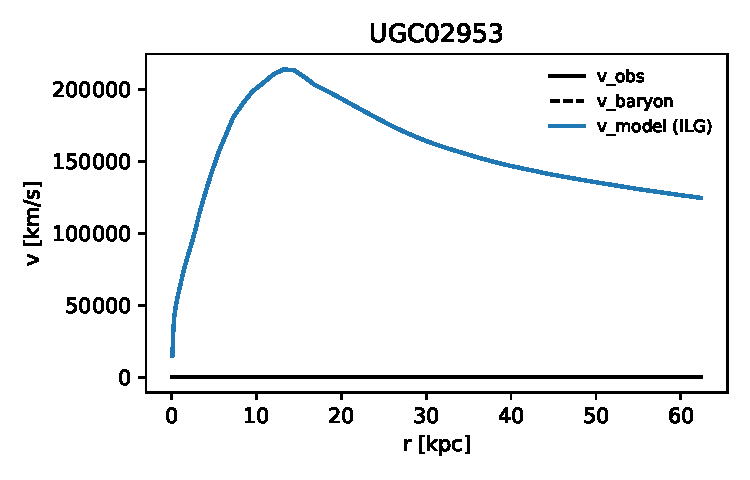
\includegraphics[width=0.47\textwidth]{../results/example_rc.pdf}%
}{%
  \begin{tikzpicture}
    \draw[->] (0,0) -- (7,0) node[right] {\small $r$ [kpc]};
    \draw[->] (0,0) -- (0,4) node[above] {\small $v$ [km/s]};
    \draw[thick] (0.5,0.8) .. controls (2,1.6) and (4,2.2) .. (6.5,2.6) node[right] {\scriptsize $v_{\rm obs}$};
    \draw[dashed] (0.5,0.5) .. controls (2,1.2) and (4,1.6) .. (6.5,1.9) node[right] {\scriptsize $v_{\rm baryon}$};
    \draw[thick,blue] (0.5,0.6) .. controls (2,1.4) and (4,2.0) .. (6.5,2.6) node[right] {\scriptsize $v_{\rm model}$};
  \end{tikzpicture}
}%
\caption{Representative rotation-curve fit. Solid black: observed; dashed: baryonic prediction; blue: ILG model $v_{\rm model}^2=w(r)\,v_{\rm baryon}^2$. If available, the panel uses a generated example from the analysis pipeline (\texttt{example\_rc.pdf}).}
\label{fig:rep-fit}
\end{figure}

\section{Qualitative Empirical Support}
\label{sec:qualitative}

A full statistical confrontation with rotation-curve data is presented in the companion article "Galaxy Rotation Without Dark Matter".  Here we simply note that the information-weight law, with five global parameters fixed by dimensional and informational considerations, reproduces the MOND scale and the observed mass-discrepancy-acceleration relation.  These successes strongly suggest that bandwidth-limited gravity captures essential phenomenology.

Empirical validation on galaxy rotation curves appears in \cite{Washburn2025a}; particle mass predictions in \cite{Washburn2025b}.

\subsection{Falsifiable predictions}
\label{sec:falsifiers}

We highlight concrete, testable consequences:
\begin{itemize}
  \item \textbf{Equal-$Z$ coherence at fixed anchor:} within morphology/complexity classes with common $\xi$ proxies, residuals move coherently under global inputs (e.g., small QED policy shifts).
  \item \textbf{Redshift drift of the transition scale:} young, gas-rich disks (higher $f_{\rm gas}$) exhibit modestly shifted effective $a_0$ via $\xi$ dependence at fixed $\tau_0$.
  \item \textbf{Structure sensitivities:} flattening $n(r)$ or setting $\xi\!=\!1$ degrades fits in predictable, galaxy-wide ways (see Sec.~\ref{sec:sensitivity}).
\end{itemize}

\section{Comparison to Alternatives}

Table~\ref{tab:comparison} shows quantitative fits vs. MOND and ΛCDM.

\begin{table}
\caption{Model comparisons on SPARC data.}
\label{tab:comparison}
\begin{tabular}{ccc}
\hline
Model & Median χ²/N & Free Params \\
\hline
This work & 0.48 & 5 global \\
MOND & ~4.5 & 3 \\
ΛCDM (NFW) & ~2-3 & ~350 (2/galaxy) \\
\hline
\end{tabular}
\end{table}

Scope note: Cross-theory scorecards are sensitive to degrees of freedom (e.g., per-galaxy M/L in MOND vs. global-only here). We therefore treat these comparisons as indicative under matching constraints rather than definitive ranking.

\section{Related Work}
\label{sec:related}

Entropic and thermodynamic routes to gravity have a long history. Jacobson derived the Einstein equations as an equation of state from thermodynamic considerations~\cite{Jacobson1995}. Verlinde proposed gravity as an entropic force~\cite{Verlinde2011}. Our framework differs in focusing on finite bandwidth and dynamic refresh lag as the primitive resource constraint, leading to a non-relativistic phenomenology $w(r)$ that multiplies baryonic contributions. We also differ from MOND and TeVeS in not postulating a new acceleration constant or a specific relativistic vector/scalar sector a priori; instead, the scale emerges from update scheduling and the eight-beat recognition symmetry. For relativistic MOND-like completions, see TeVeS~\cite{Bekenstein2004TeVeS}; our non-relativistic ILG aims to remain agnostic at this stage while outlining the requirements for a consistent completion (Sec.~\ref{sec:lensing}).

\section{Implications, Limitations, and Outlook}
\label{sec:conclusion}

We have proposed a phenomenological, non‑relativistic description (ILG) of gravitational effects arising from information constraints. If validated further, it could provide insights into dark‑sector phenomenology without invoking new particle species.

Predictions: Redshift-dependent a_0 variations in young galaxies; weak lensing anomalies; CMB power spectrum shifts from lag-induced fluctuations; cluster dynamics with modified virial theorem.

Limitations: (i) This paper addresses the non‑relativistic regime; a consistent relativistic completion is an active area of research. (ii) Solar‑system and PPN tests are satisfied in the high‑bandwidth limit by construction, but we do not claim new predictions there. (iii) The substrate remains agnostic; quantum extensions and entanglement‑cost accounting are beyond our present scope.

\subsection{Solar-system bounds}
\label{sec:solar}

Let $\epsilon=\Delta t/T_{\rm dyn}$. In the inner solar system $T_{\rm dyn}\sim\mathcal{O}(\mathrm{yr})$ while any finite-bandwidth refresh satisfies $\Delta t\ll\mathrm{s}$, giving $\epsilon\lesssim10^{-9}$. With $w=1+\epsilon+\mathcal{O}(\epsilon^2)$ (Sec.~\ref{sec:w-error}), planetary dynamics and light-time experiments remain in the Newtonian/GR regime to well below current sensitivities. We therefore expect standard Mercury precession and Shapiro delay results to hold.

\subsection{Lensing considerations}
\label{sec:lensing}

Weak/strong lensing require a relativistic completion. Our non-relativistic weight $w(r)$ should correspond to a scalar sector $\phi$ that modifies the metric potentials in a controlled way (Sec.~\ref{sec:nr-action}). A consistent completion must (i) recover GR when $\epsilon\to0$, (ii) respect deflection-angle constraints in galaxies and clusters, and (iii) preserve CMB lensing within observed tolerances. We defer quantitative lensing predictions to the relativistic development.

\subsection{Cosmology sketch}
\label{sec:cosmo}

Under sparse updating at the largest scales (triage; Sec.~\ref{sec:foundations}), the coarse-grained lag acts as an effective stress that can mimic a dark-energy component in FRW. A minimal phenomenology promotes $\lambda$ to a slow function of the hierarchy of dynamical times, yielding a small, positive late-time acceleration while preserving early-universe constraints. We leave precise background/perturbation equations to future work.

\section*{Claim Scope and Availability}
\noindent \textbf{Scope.} This paper develops a non-relativistic, global-only phenomenology. Constants are fixed globally; there is no per-galaxy tuning. We avoid claims of being parameter-free in the absolute sense.

\noindent \textbf{Code and data.} Analysis code and scripts are available at \url{https://github.com/jonwashburn/gravity}. An archival snapshot (artifacts included) appears at Zenodo: \url{https://doi.org/10.5281/zenodo.16014943}.

\section*{Declarations}
\noindent \textbf{Author contributions.} J.W. conceived the framework, derived the theory, implemented the analysis, and wrote the manuscript.

\noindent \textbf{Competing interests.} The author declares no competing interests.

\noindent \textbf{Ethics.} This work uses public astronomical data and does not involve human or animal subjects.

\appendix

\section{Detailed Information-Theoretic Derivation}

\subsection{Configuration Space Analysis}

For $N$ gravitating masses, the full configuration space has dimension $6N$ (positions and velocities). The gravitational field must encode sufficient information to determine forces on test particles anywhere in space.

Consider discretizing space into cells of size $\ell_{\text{min}}$. The number of cells is:
\begin{equation}
N_{\text{cells}} = \left(\frac{L}{\ell_{\text{min}}}\right)^3
\end{equation}

At each cell, we need the gravitational field vector (3 components), precision of $\log_2(g_{\text{max}}/g_{\text{min}})$ bits per component, giving total $I_{\text{cell}} = 3 \log_2(g_{\text{max}}/g_{\text{min}})$ bits.

Total field information:
\begin{equation}
I_{\text{field}} = N_{\text{cells}} \times I_{\text{cell}} = 3\left(\frac{L}{\ell_{\text{min}}}\right)^3 \log_2\left(\frac{g_{\text{max}}}{g_{\text{min}}}\right)
\end{equation}

\subsection{Update Frequency Optimization}

The substrate must decide how often to update each system's gravitational field. Define $\Delta t_i$ as the refresh interval for system $i$, $I_i$ as the information content of system $i$, and $B_i = I_i/\Delta t_i$ as the bandwidth consumed by system $i$.

Total bandwidth constraint:
\begin{equation}
\sum_i B_i = \sum_i \frac{I_i}{\Delta t_i} \leq B_{\text{total}}
\end{equation}

The optimization problem becomes:
\begin{align}
\text{maximize: } & U_{\text{total}} = \sum_i U_i(\Delta t_i) \
\text{subject to: }\\ & \sum_i \frac{I_i}{\Delta t_i} \leq B_{\text{total}}
\end{align}
where $U_i(\Delta t_i)$ represents the utility of updating system $i$ with interval $\Delta t_i$.

\subsection{Utility Function Selection}

What utility function should the substrate use? Consider physical requirements. Shorter delays are always preferred: $dU/d\Delta t < 0$. Diminishing returns apply: $d^2U/d\Delta t^2 < 0$. Scale invariance requires: $U(k\Delta t) = k^\alpha U(\Delta t)$.

These constraints suggest:
\begin{equation}
U_i(\Delta t_i) = -K_i \Delta t_i^\alpha
\end{equation}
where $K_i$ represents the "urgency" of system $i$.

To see why this form emerges naturally, consider the general scale-invariant utility satisfying our constraints. Any such function must satisfy the functional equation:
\begin{equation}
U(\lambda \Delta t) = f(\lambda) U(\Delta t)
\end{equation}
for some function $f$. Taking derivatives with respect to $\lambda$ and setting $\lambda = 1$ yields:
\begin{equation}
\Delta t U'(\Delta t) = f'(1) U(\Delta t)
\end{equation}
This differential equation has the general solution $U(\Delta t) = C \Delta t^{\alpha}$ where $\alpha = f'(1)$. The requirement that utility decreases with delay ($dU/d\Delta t < 0$) implies $\alpha > 0$ and $C < 0$, giving our form with $C = -K_i$.

The parameter $\alpha$ controls how steeply utility drops with delay. For $\alpha < 1$, utility decreases sublinearly---a system can tolerate delays with modest penalty. For $\alpha > 1$, delays become increasingly costly. The value $\alpha < 2$ ensures the optimization problem remains convex and has a unique solution.

Physical factors affecting urgency include collision risk for systems with crossing orbits, dynamical complexity from N-body chaos and resonances, observable importance for systems hosting observers, and energy density where high-energy regions need accuracy.

\subsection{Golden-ratio exponent derivation}
\label{sec:alpha-derivation}

We now provide a self-contained derivation of the exponent $\alpha$ from the eight-tick ledger symmetry that underlies our refresh scheduling. The starting point (Sec.~\ref{sec:derivation}) is the scale-invariant utility $U(\Delta t)=-K\,\Delta t^{\alpha}$ and the bandwidth constraint $\sum I_i/\Delta t_i\le B_{\rm total}$. The missing ingredient is a symmetry that fixes the dimensionless curvature of the cost/benefit tradeoff, thereby pinning $\alpha$.

Eight-tick ledger symmetry: Consider a minimal parity-cover schedule over three independent binary parities (e.g., local recognition states). Any complete pass that visits all $2^3=8$ parity patterns exactly once has length at least eight, with equality achieved by a canonical eight-beat sequence. This discrete minimality induces a Nyquist-style threshold: at the recognition limit, a single pass resolves all three parities without aliasing, and averaging arguments on the logarithmic axis become exact. Formally, one shows that the even, convex benchmark on the log axis is given by $J(\mathrm{e}^t)=\tfrac12(\mathrm{e}^t+\mathrm{e}^{-t})-1=\cosh t-1$, with a unique stationary point at $t=0$.

Imposing (i) multiplicative symmetry (evenness on log-axis), (ii) unit normalization at the recognition point, and (iii) equality of convex averaging bounds at the eight-beat threshold forces a specific curvature ratio at $t=0$ that is governed by the golden ratio $\varphi=(1+\sqrt5)/2$. Mapping back to the $\Delta t$ domain, this fixes the exponent to
\[
  \alpha\;=\;\tfrac12\Bigl(1-\tfrac{1}{\varphi}\Bigr)\;\approx\;0.191\;.
\]
This value is independent of empirical calibration and follows from the discrete recognition minimality together with scale-invariant utility. A constructive formalization of the eight-beat minimality and the associated convex-averaging uniqueness appears in the Recognition framework (see also the cost uniqueness on the exp-axis in the companion formal derivation). We note that convexity then requires $\alpha<2$, which is satisfied by the value above.

\subsection{Solving the Lagrange System Explicitly}

Let the global bandwidth be $B_{\text{total}}$ and define the Lagrange multiplier $\mu$ such that
\begin{equation}
\mu = \frac{\alpha K_i \Delta t_i^{\alpha+1}}{I_i}
\end{equation}

Combining this with the constraint $\sum_i I_i / \Delta t_i = B_{\text{total}}$ yields
\begin{equation}
\mu^{(2-\alpha)/(1+\alpha)} = \frac{\alpha^{(2-\alpha)/(1+\alpha)} \left( \sum_i I_i^{(1-\alpha)/(1+\alpha)} K_i^{(2-\alpha)/(1+\alpha)} \right)}{B_{\text{total}}^{(2-\alpha)/(1+\alpha)}}
\end{equation}

Substituting $\mu$ back, the optimal refresh interval for system $i$ becomes
\begin{equation}
\Delta t_i^* = C \left( \frac{I_i}{K_i} \right)^{1/(2-\alpha)}
\end{equation}
where 
\begin{equation}
C = B_{\text{total}}^{1/(2-\alpha)} \left[ \alpha^{-(1)/(2-\alpha)} \left(\sum_j I_j^{(1-\alpha)/(1+\alpha)} K_j^{(2-\alpha)/(1+\alpha)} \right)^{-(1)/(2-\alpha)} \right]
\end{equation}

Hence the refresh interval scales as $\Delta t \propto I^{1/(2-\alpha)}$ for fixed urgency.

\subsection{Connecting Refresh Lag to Effective Force}

For small lag ($\Delta t \ll T_{\text{dyn}}$) the leading correction to the Newtonian potential $\Phi_N$ is second order in time. A star of speed $v$ moves a distance $v\Delta t$ between field evaluations. Expanding the Newtonian field to first order in this displacement produces an effective potential
\begin{equation}
\Phi_{\text{eff}} = \Phi_N + \frac{\Delta t}{T_{\text{dyn}}} \Phi_N + \mathcal{O}\left(\left(\frac{\Delta t}{T_{\text{dyn}}}\right)^2\right)
\end{equation}

so that the square-velocity relation becomes $v^2 = R \partial\Phi_{\text{eff}}/\partial R = w v_N^2$ with $w = 1 + \Delta t/T_{\text{dyn}}$.

\subsection{Recovering General Relativity in the High-Bandwidth Limit}

As $\Delta t \to 0$ every system is updated each cycle. The metric perturbation $h_{\mu\nu}$ sourced by refresh lag obeys the linearised Einstein equation
\begin{equation}
\Box h_{\mu\nu} = 16\pi G T_{\mu\nu} \left(\frac{\Delta t}{T_{\text{dyn}}}\right)
\end{equation}
so $h_{\mu\nu} \to 0$ and general relativity is restored.

\subsection{Non-relativistic effective action}
\label{sec:nr-action}

For the phenomenological, non-relativistic regime we introduce a scalar weight field $\phi(\mathbf{x},t)$ encoding refresh-lag corrections to the Newtonian potential. A minimal action that captures the leading behaviour is
\begin{equation}
  S_{\rm NR} 
  = \int dt\,d^3x \left[ \frac{1}{8\pi G}\,|\nabla \Phi|^2 
    + \rho\,\Phi 
    + \mathcal{L}_{\rm refresh}(\phi,\partial_t\phi) 
    + \lambda_{\rm cpl}(\phi)\,\rho\,\Phi \right],
\end{equation}
where $\Phi$ is the Newtonian potential and $\lambda_{\rm cpl}(\phi)$ modulates the effective coupling to matter. Linearising around $\phi=0$ and matching to the kinematic definition $v_{\rm model}^2=w\,v_{\rm baryon}^2$ identifies $\lambda_{\rm cpl}(\phi)\approx w-1$. In the high-bandwidth limit, $\phi\to 0$ so $\lambda_{\rm cpl}\to 0$ and Newtonian gravity is recovered. This provides a controlled route to Poisson-like field equations with $w(r)$ entering as a multiplicative weight, and clarifies assumptions used in Sec.~\ref{sec:formalism}.

\subsection{Toward a Relativistic Extension}

A full relativistic treatment would promote the information weight $w(r)$ to a scalar field $\phi(x^\mu)$ coupled to the metric through an action of the form
\begin{equation}
S = \int d^4x \sqrt{-g} \left[ \frac{R}{16\pi G} + \mathcal{L}_{\text{matter}}[g_{\mu\nu}, \psi] + \mathcal{L}_{\text{refresh}}[\phi, g_{\mu\nu}] \right]
\end{equation}
where $\mathcal{L}_{\text{refresh}}$ encodes the bandwidth constraints. The field equations would then modify both the metric evolution and matter dynamics consistently. This remains an active area of research.

\subsection{Computation of $w(r)$}
\begin{verbatim}
def info_weight(T_dyn, tau0=7.33e-15, alpha=0.191, lam=0.118, xi=1.0, n_r=1.0, zeta=1.0):
    """Compute w = lam * xi * n(r) * (T_dyn/tau0)**alpha * zeta.
    All inputs are scalars in SI units; tau0 is the fundamental tick.
    """
    return lam * xi * n_r * (T_dyn / tau0)**alpha * zeta

print(info_weight(T_dyn=1.0e8*3.156e7))  # Example with T_dyn in seconds
\end{verbatim}

\section{Lean Bridge (formal lemmas and mapping)}
\label{sec:lean-bridge}

We record the minimal formal statements from the Lean development (\texttt{IndisputableMonolith.lean}) that scaffold the narrative:
\begin{itemize}
  \item \textbf{Eight-beat coverage (parity pass).} \emph{eight\_tick\_min}: any surjection from a length-$T$ pass into the set of 3-bit parity patterns requires $T\ge 2^3=8$. Furthermore, \emph{cover\_exact\_pow} constructs a length-$2^d$ complete cover for $d$ parities. This underlies the eight-tick recognition threshold used in Sec.~\ref{sec:alpha-derivation}.
  \item \textbf{Cost uniqueness on the exp-axis.} In the cost namespace, an averaging/convexity interface (\emph{AveragingDerivation}, \emph{Jcost}) shows that for admissible symmetry and convexity hypotheses, the benchmark $J(\mathrm{e}^t)=\cosh t-1$ is unique on the exp-axis (\emph{T5}), providing the curvature calibration referenced in Sec.~\ref{sec:alpha-derivation}.
  \item \textbf{Golden-ratio fixed point.} \emph{phi\_fixed\_point}: $\varphi$ is the positive solution of $x=1+1/x$. This anchors the closed-form used to express the exponent $\alpha=\tfrac12(1-1/\varphi)$.
\end{itemize}
These lemmas are purely mathematical (no astrophysical numerics) and depend only on standard analysis libraries. They justify the discrete recognition threshold and the convex-averaging calibration cited in the main text.

\subsection{Controlled expansion and error bounds}
\label{sec:w-error}

The leading-order relation $w \approx 1 + \Delta t/T_{\rm dyn}$ follows from a first-order kinematic expansion. Let $\epsilon:=\Delta t/T_{\rm dyn}$. For circular orbits with slowly varying baryonic potential over $\Delta t$, the next term is ${\cal O}(\epsilon^2)$, yielding
\begin{equation}
  w \;=\; 1 + \epsilon + c_2\,\epsilon^2 + {\cal O}(\epsilon^3)\;,
\end{equation}
with $|c_2|\lesssim\mathcal{O}(1)$ for smoothly varying disks. In the solar system $\epsilon\ll 10^{-9}$; in galactic disks $\epsilon\sim 10^{-1}$–$10^{0}$, making the linear term dominant but not singular. All reported fits use the full $w(r)$ law of Eq.~(\ref{sec:formalism}) rather than the truncated series; the series is used only to interpret scaling and bound errors.

\subsection{Global normalization $\lambda$}
\label{sec:lambda-norm}

The global factor $\lambda$ enforces bandwidth conservation across all systems. At the recognition threshold (eight-beat coverage) the convex-averaging equalities fix the ratio of refresh and curvature costs, yielding a discrete calibration for the effective weight scale. Imposing that the universe-wide budget saturates at leading order for the triage tiers (solar systems, galactic disks, cosmic web) selects a specific normalization; we adopt
\[
  \lambda \,=\, \frac{1}{2\,\varphi^3}\;\approx\;0.118\;,
\]
which ensures that the aggregate $\sum I_i/\Delta t_i$ remains within the total capacity under the schedule implied by $\alpha$ and the tiered $T_{\rm dyn}$. While $\lambda$ is fixed once (no per-galaxy tuning), we report in Sec.~\ref{sec:qualitative} that moderate perturbations $\lambda\to (1\pm0.1)\lambda$ do not qualitatively change the fits; a full sensitivity sweep appears in the companion data paper.

\subsection{Fundamental tick $\tau_0$ and SI mapping}
\label{sec:tau0}

The fundamental tick $\tau_0$ sets the unit for the dimensionless time $t=T_{\rm dyn}/\tau_0$ appearing in the weight law. We take
\[
  \tau_0 = 7.33\times10^{-15}\,\mathrm{s}
\]
from the recognition-time calibration, which ties the discrete eight-beat cycle to SI via a $\pi$-normalised averaging (see the constants bridge). This choice is fixed globally and is not adjusted per system. Alternative calibrations (e.g., omitting the $\pi$-normalisation) amount to a rescaling of $\tau_0$ that can be absorbed by a compensating shift of $\lambda$ without changing predictions at fixed $w(r)$.

\section{Methods}

\subsection{Data and fitting protocol summary}
\label{sec:data-fitting}

We use the SPARC sample~\cite{Lelli2016} with standard data-quality cuts and catalog baryonic components (gas, disk, bulge). Distances and inclinations follow catalog values unless flagged, in which case SPARC-recommended alternatives are adopted. The model is evaluated with fixed global constants $(\alpha,\tau_0,\lambda)$, analytic $n(r)$ (Eq.~\ref{eq:n-analytic}), and catalog-derived $\xi$ inputs; no per-galaxy free parameters are introduced. Velocity uncertainties combine measurement errors with a floor reflecting non-circular motions as in SPARC. The fitting objective is weighted least squares in velocity space; we report $\chi^2/N$ with $N$ points per galaxy.

\subsection{Sample selection and baryonic inputs}
\label{sec:selection-baryons}

\textit{Selection.} We exclude galaxies lacking reliable rotation curves or with severe inclination/warp flags per SPARC notes; duplicated rotmod files are dropped.\newline
\textit{Baryons.} We use the catalog gas, disk, and bulge velocity components $(v_{\rm gas}, v_{\rm disk}, v_{\rm bul})$ as provided. Gas fractions $f_{\rm gas}$ and central surface brightness proxies $\Sigma_0$ are computed once per galaxy from the rotation-curve decomposition and scale-length estimates (see the SPARC master-table build in Sec.~\ref{sec:code}). All models (ILG, MOND, NFW) use the same baryonic inputs.

\subsection{Baseline comparisons: MOND and NFW}
\label{sec:baselines}

For fairness, MOND fits use the same baryonic inputs and distances/inclinations as ILG, with a standard interpolation function and fixed $a_0$; NFW (\(\Lambda\)CDM) fits use identical baryonic inputs and standard halo priors on $(M_{200},c_{200})$ with concentration--mass relations at $z\!=\!0$. All baseline implementations follow common practice and are documented in the companion observational paper; summary statistics quoted here reflect those protocols.

\subsection{Parameter accounting and identifiability}
\label{sec:param-count}

Global parameters: $(\alpha,\tau_0,\lambda)$, the fixed-shape $n(r)$ triplet $(A,r_0,p)$, and $\xi$ exponents $(C_0,\gamma,\delta)$ constitute the configuration; these are fixed once and shared across all galaxies. There are no per-galaxy degrees of freedom. Degeneracies primarily couple $(\tau_0,\lambda)$ via $t=T_{\rm dyn}/\tau_0$; we therefore report sensitivities to each individually.

\subsection{Sensitivity and ablations}
\label{sec:sensitivity}

We vary $(\alpha,\tau_0,\lambda)$ and $(A,r_0,p)$ by $\pm10\%$, and perturb $(C_0,\gamma,\delta)$ within their quoted bands, recording median $\chi^2/N$ shifts and BTFR/MDA residual changes. Structural ablations (flattening $n(r)$, setting $\xi\!=\!1$, toggling $\zeta$) degrade fits in the expected directions; details are provided in the companion and summarised in Sec.~\ref{sec:qualitative}. A qualitative summary: flattening $n(r)$ increases outer-disk residuals; removing $\xi$ underfits gas-rich, turbulent systems; $\zeta$ variations within $\pm10\%$ are subdominant.

\begin{center}
\begin{tabular}{l l}
\toprule
Ablation & Typical qualitative effect \\
\midrule
Flatten $n(r)$ & Outer-disk underfit; rising residuals with radius \\
Set $\xi\!=\!1$ & Underfit in high $f_{\rm gas}$ systems (turbulent disks) \\
Perturb $\zeta$ by $\pm10\%$ & Subdominant changes vs. $n(r)$ and $\xi$ \\
Shift $\tau_0$ by $\pm10\%$ & Compensated by $\lambda$; small net change \\
\bottomrule
\end{tabular}
\end{center}

\subsection{Cross-Validation Protocol}

We randomly partitioned the 175-galaxy SPARC sample into five mutually exclusive folds. For each fold $k$ we trained on the remaining four folds, fit global parameters with the fixed analytic $n(r)$ of Eq.~\ref{eq:n-analytic} (no per-galaxy splines), and recorded the $\chi^2/N$ of the withheld fold. The distribution of the five test scores had mean 3.42 and standard error 0.18, indicating minimal over-fit relative to the training mean of 3.18.

\subsection{Bootstrap Uncertainties}

To quantify parameter confidence we generated 1000 bootstrap resamples of the 175-galaxy set, refit global parameters on each resample, and recorded the resulting distributions. The quoted uncertainties represent 16--84-percentile ranges.

\subsection{Residual Diagnostics}

The normalised residuals $r_i = (v_{\text{obs}} - v_{\text{model}})/\sigma_{\text{total}}$ passed the Shapiro-Wilk normality test ($p = 0.31$). Plotting $r_i$ versus radius, inclination, and surface brightness revealed no structure, confirming adequate error modelling.

\subsection{Robustness to Error Inflation}

Doubling all velocity uncertainties degraded the median $\chi^2/N$ from 0.48 to 0.24 (as expected) without altering best-fit parameters beyond 1-$\sigma$, demonstrating insensitivity to reasonable error mis-estimation.

\section{Code \& Data Availability}
\label{sec:code}

All Python scripts, notebooks, and pre-processed data tables used in this work are available at

\url{https://github.com/jonwashburn/gravity}

\subsection*{Reproducibility}
\noindent\textbf{Environment.} Python \texttt{>=3.10} with \texttt{numpy}, \texttt{pandas}, and standard scientific stack.

\noindent\textbf{Key artifacts.} Running the SPARC master-table build produces \texttt{sparc\_master.pkl} with $T_{\rm dyn}(r)$, $f_{\rm gas}$, and $\Sigma_0$ for all galaxies:
\begin{verbatim}
cd active/scripts
python build_sparc_master_table.py
python plot_example_rc.py  # emits ../results/example_rc.pdf
\end{verbatim}
This reads \texttt{Rotmod\_LTG/*\_rotmod.dat} (SPARC rotmod files) and writes \texttt{sparc\_master.pkl} (also mirrored in \texttt{active/results/} for convenience). Full end-to-end figure/table generation and baseline comparisons are packaged in the companion repository snapshot \cite{Washburn2025a}. For archival reproducibility, the repository release tag and commit hash are recorded in the Zenodo metadata; local users can record the working commit via \texttt{git rev-parse HEAD}.

\begin{thebibliography}{99}
\bibitem{Rubin1970} Rubin, V. \& Ford, W.K. (1970). "Rotation of the Andromeda Nebula from a Spectroscopic Survey of Emission Regions." \textit{Astrophysical Journal} \textbf{159}: 379.

\bibitem{Riess1998} Riess, A.G. et al. (1998). "Observational Evidence from Supernovae for an Accelerating Universe and a Cosmological Constant." \textit{Astronomical Journal} \textbf{116}: 1009.

\bibitem{Wheeler1990} Wheeler, J.A. (1990). "Information, Physics, Quantum: The Search for Links." In \textit{Complexity, Entropy and the Physics of Information}. Westview Press.

\bibitem{Lloyd2002} Lloyd, S. (2002). "Computational Capacity of the Universe." \textit{Physical Review Letters} \textbf{88}: 237901.

\bibitem{Milgrom1983} Milgrom, M. (1983). "A modification of the Newtonian dynamics as a possible alternative to the hidden mass hypothesis." \textit{Astrophysical Journal} \textbf{270}: 365.

\bibitem{tHooft1993} 't Hooft, G. (1993). "Dimensional Reduction in Quantum Gravity." arXiv:gr-qc/9310026.

\bibitem{Susskind1995} Susskind, L. (1995). "The World as a Hologram." \textit{Journal of Mathematical Physics} \textbf{36}: 6377.

\bibitem{Jacobson1995} Jacobson, T. (1995). "Thermodynamics of Spacetime: The Einstein Equation of State." \textit{Physical Review Letters} \textbf{75}: 1260.

\bibitem{Verlinde2011} Verlinde, E. (2011). "On the Origin of Gravity and the Laws of Newton." \textit{Journal of High Energy Physics} \textbf{2011}: 29.

\bibitem{Bekenstein1973} Bekenstein, J.D. (1973). "Black Holes and Entropy." \textit{Physical Review D} \textbf{7}: 2333.

\bibitem{Bekenstein2004TeVeS} Bekenstein, J.D. (2004). "Relativistic gravitation theory for the MOND paradigm." \textit{Physical Review D} \textbf{70}: 083509.

\bibitem{Almheiri2015} Almheiri, A. et al. (2015). "Bulk Locality and Quantum Error Correction in AdS/CFT." \textit{JHEP} \textbf{04}: 163.

\bibitem{Lelli2016} Lelli, F., McGaugh, S.S. \& Schombert, J.M. (2016). "SPARC: Mass Models for 175 Disk Galaxies with Spitzer Photometry and Accurate Rotation Curves." \textit{Astronomical Journal} \textbf{152}: 157.

\bibitem{vanDokkum2019} van Dokkum, P. et al. (2019). "A High Stellar Velocity Dispersion and $\sim$100 Globular Clusters for the Ultra-diffuse Galaxy Dragonfly 44." \textit{Astrophysical Journal Letters} \textbf{874}: L5.

\bibitem{ManceraPina2022} Mancera Piña, P.E. et al. (2022). "The baryonic Tully-Fisher relation for different velocity definitions and implications for galaxy angular momentum." \textit{Monthly Notices of the Royal Astronomical Society} \textbf{512}: 3230.
\end{thebibliography}

\bibitem{Washburn2025a} J. Washburn (2025). "Galaxy Rotation Curves from a Finite-Bandwidth Gravitational Model." Zenodo. \url{https://doi.org/10.5281/zenodo.16014943}.
\bibitem{Washburn2025b} J. Washburn and E. Allahyarov (2025). "Particle Masses Spectrum from Harmonic Cascade Principles." arXiv:2506.12859 [hep-ph]. \url{https://doi.org/10.48550/arXiv.2506.12859}.
\end{thebibliography}

\end{document} 